\chapter{TROPOS Methodology with Probabilistic Requirements Verification}\label{ch:proposal}

This chapter describes the extended TROPOS methodology applied to the MPERS case study. Both TROPOS early and late requirements analysis phases are fully presented, as long as the verification process that requires a behaviour specification and the additional contextual notation regarding context effects. Further details about the TROPOS methodology may be found in the reference literature~[TROPOS]. 

\section{TROPOS Requirements Engineering Phases}

\subsection{TROPOS Early Requirements Phase}

In Early Requirements phase, stakeholders are modelled as as well as their needs. Each actor may be a depender or a dependee of a goal, task or resource dependency. In this phase, only the main system actor and the application domain stakeholders are analysed, leaving the detailed system analysis to later development phases.

The MPERS sytem and its social dependencies are presented by the actor model in Figure~\ref{fig:MPERS_ER}. System actors and social actors are displayed in different colors. Among the stakeholders, the emergency center represents a private or public organization interested in providing an emergency response service to patients. Patient and doctor represent, respectively, the assisted person and the medical responsible for defining and evolving the emergency detection rules as part of an evolutionary approach for personal emergency response. Finally, sensors retailer should provide the vital signs sensors required for monitoring.

\begin{figure*}[ht]
\centering
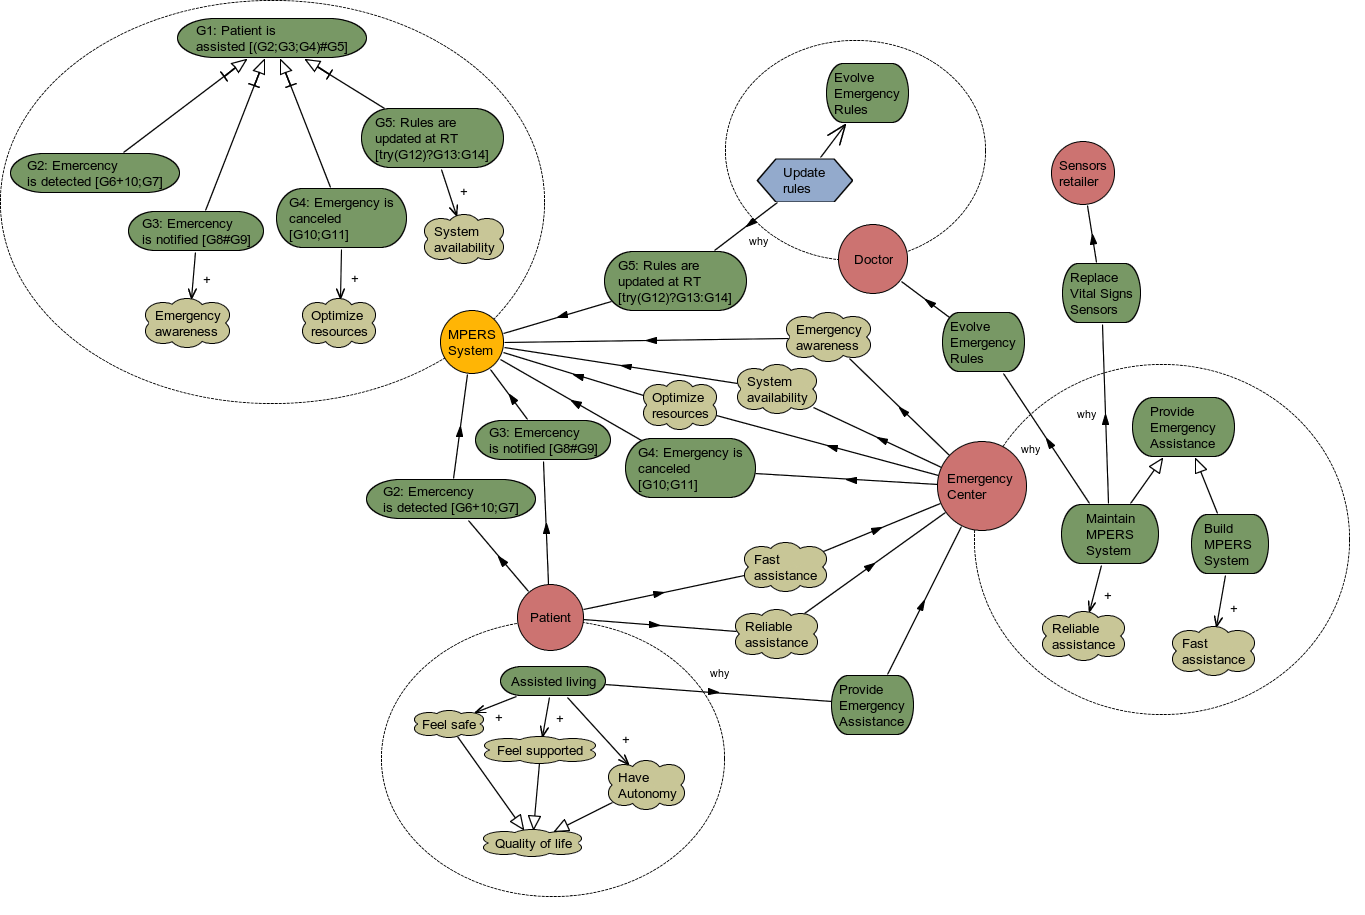
\includegraphics[width=1\textwidth]{imgs/MPERS_ER.png}
\caption{MPERS at TROPOS early requirements phase}
\label{fig:MPERS_ER}
\end{figure*}

From the diagram in Figure~\ref{fig:MPERS_ER} it is possible to have a first view of the MPERS system-to-be. Main goals are divided in detecting, notifying and checking an emergency. Also, the ability to update the emergency rules at runtime (RT) is the fourth and last mandatory goal (AND-decomposition) that fulfils the `Patient is assisted' root goal. System goals are directly or indirectly related to stakeholders functional and non-functional needs.

The yellow circle indicates that MPERS is a system actor. MPERS goals can be seen with a regex indicating its dynamic behaviour as part of the runtime goal model specification required by the proposal. This notation is a reflex of the late requirements phase, as the TAOM4E tool supporting TROPOS methodology shares unique entities and relations among different development phases. The regex syntax is enclosed by brackets to differentiate then from goal name. In future work, a specific modelling compartment should receive the values for the runtime regex.

\subsection{TROPOS Late Requirements Phase}

Later requirements phase concentrates the analysis in the system-to-be and its operational environment. The MPERS goal model occupies the most part of the diagram and each of its main goals are further decomposed through AND/OR decomposition. Also, means-end tasks defines how leaf-goals are fulfilled and the runtime regex across goals and tasks specifies dynamic properties of the system-to-be behaviour. Figure~\ref{fig:MPERS_LR} illustrates the late requirements diagram for the MPERS.

\begin{figure*}[h!]
\centering
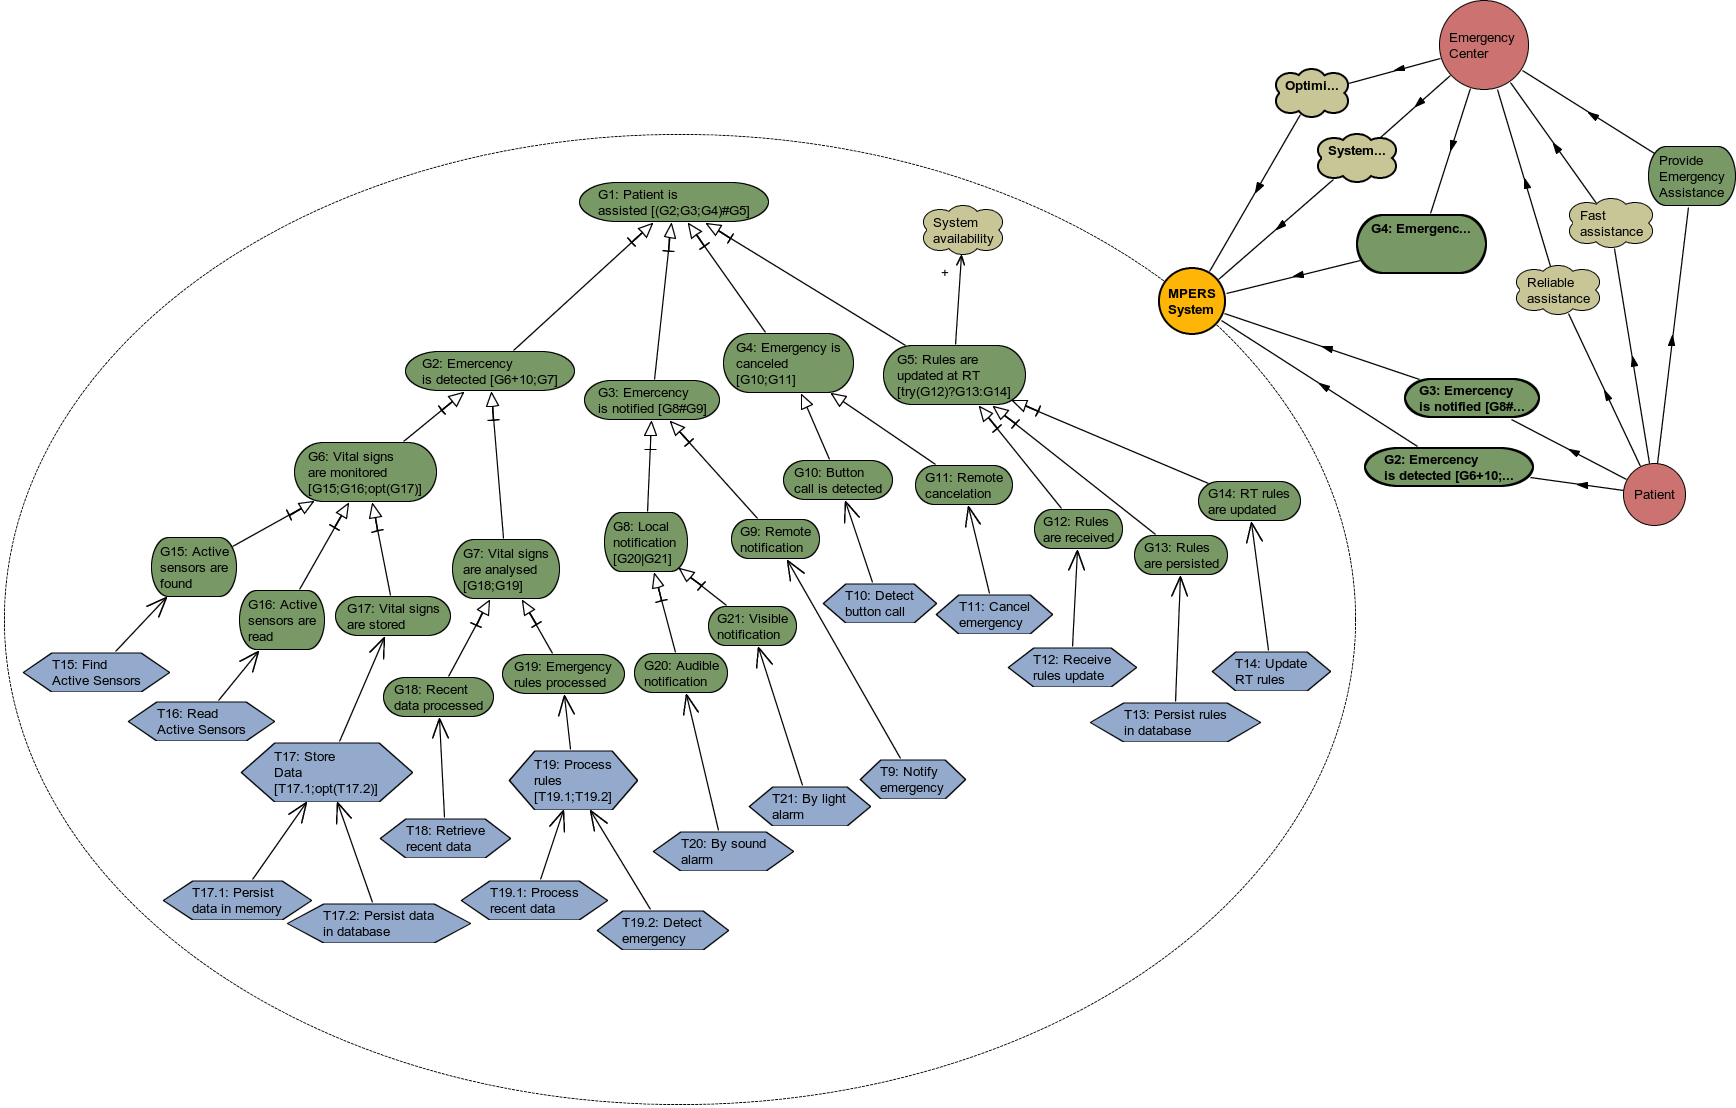
\includegraphics[width=1\textwidth]{imgs/MPERS_LR.png}
\caption{MPERS at TROPOS early requirements phase}
\label{fig:MPERS_LR}
\end{figure*}

At this stage of the methodology, the system is represented as a monolithic actor and its goal model may be extended with the runtime specification. This extended model merges multiple views in the same diagram: goals and tasks represent the requirements view for the system-to-be as well as the intentionality behind then, while the runtime specification provides a dynamic representation in terms of goal achievement  and task execution.

In this work, we have first explored the use of the PMC technique for the verification of dependability attributes in the system model of the TROPOS late requirements phase. The idea is to initially evaluate the approach in a monolithic representation without the additional complexity of a multi-agent architecture. The evaluation involving later TROPOS phases should be explored in future work. The remaining of this section will focus on the extended verification phase proposed by this work.

\section{TROPOS Extended Verification Phase}

To evaluate our verification approach with the MPERS case study, we have used a discrete-time Markov chain (DTMC) probabilistic model and focused on the verification of NFR related to dependability, i.e., NFR that are either direct attributes encompassed by dependability or that are related to one or more of these attributes.

\subsection{Behaviour specification}

In this section, further details about the runtime regex syntax and semantic will be explained as they are a central part of this proposal. In Figure~\ref{fig:MPERS_LR}, the regex can be seen associated to system goals and tasks, for instance, G1's regex is (G2;G3;G4)\#G5. Table~\ref{tab:RGM_REGEX} provides a textual description of each RGM notation with corresponding meaning in terms of what behaviour it specifies and also an example from the MPERS RGM. The formal and detailed description can be found in the reference publication~[RGM].

% Please add the following required packages to your document preamble:
% \usepackage{booktabs}
\begin{table}[h]\label{tab:RGM_REGEX}
{\renewcommand{\arraystretch}{1.5}
\begin{tabularx}{\textwidth}{@{}l|X|X@{}}
\toprule
\textbf{Expression} & \textbf{Meaning}                                                                   & \textbf{Example (MPERS)} \\ 
skip                & No action. Useful for conditional ternary expressions involving two elements.      & try(G10)?skip:G11        \\ 
E1;E2               & A goal/task E1 must be fulfilled/executed before E2.                               & G1;G2;G3                 \\ 
E1|E2               & Fulfillment/execution of goal/task E1 is alternative with respect to E2. & T9.1|T9.2                \\ 
opt(E)              & Fulfillment/execution of goal/task E is not mandatory.                             & opt(T17.2)               \\ 
E+n                 & Goal/task E must be fulfilled/executed n times, with n \textgreater 0.             & G22+2                    \\ 
try(E)?E1:E2        & If goal/task E succeeds, E1 must be fulfilled/executed; otherwise, E2.             & try(G10)?skip:G11        \\ 
E1\#E2              & Interleaved fulfillment/execution of goal/task E1 and E2.                          & G8\#G9                   \\ 
E\#n                & Interleaved fulfillment/execution of n instances of E, with n \textgreater 0.      & -                        \\ \bottomrule
\end{tabularx}
}
\caption{Description of RGM textual notations used by the proposal.}
\end{table}

A small variation of the original regex was employed for the E+ and E\# rules. Instead of an undetermined number of goal/task instances, analyst should provide the exact number of achievement/execution of goals/tasks. This information is required for the generation of the verification model from a RGM.

\subsection{RGM-UML activity diagram comparison}

A similar specification could be provided by an UML activity diagram with activities as leaf-tasks of the goal model. However, activity diagrams have an homogeneous granularity level and do not clearly correlate behaviour to the requirements they are meant to satisfy. In contrast to the RGM, activity diagrams denote behaviour through graphical symbols, while the RGM mixes the original goal model notation with a runtime regex. This simple notation increases the utility of a goal model diagram. Figure~\ref{fig:MPERS_UMLAD} presents an activity diagram corresponding to the MPERS RGM. 

\begin{figure*}[h!]
\centering
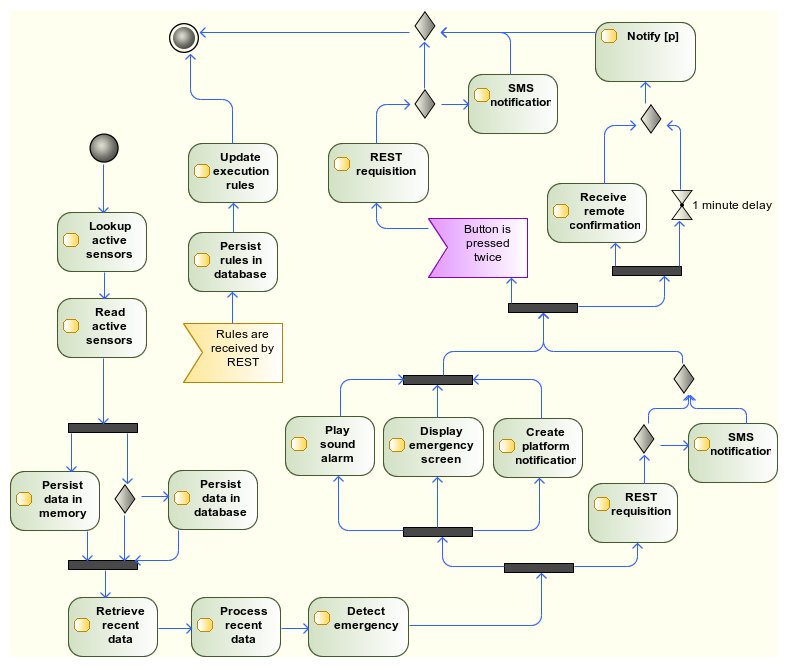
\includegraphics[width=1\textwidth]{imgs/MPERS_UMLAD.png}
\caption{MPERS tasks represented by a UML activity diagram}
\label{fig:MPERS_UMLAD}
\end{figure*}

Among its limitations, RGM does not express that an emergency has to be confirmed after a time or signal event as the UML activity diagram does. Both necessary and sufficient conditions for the triggering and fulfilment of goals, tasks and dependencies are provided by Formal TROPOS language.  Still, sequential, parallel, alternative, optional and conditional execution flows as long as multiple executions of the same task can be expressed by the RGM, providing a rich behaviour specification that could be checked for non-functional requirements such as dependability attributes.

The idea of a runtime goal model is not to replace the activity diagrams, but to empower the goal model with a clear runtime syntax that could be used for 
documentation, communication and for conformance verification at both design time and during system execution - as the execution monitoring originally proposed by Dalpiaz et al~[RGM]. Depending on the complexity of the behaviour specification, a more robust runtime syntax would have to be employed or a standard UML behaviour diagram such as activity and sequence diagrams would have to complement the goal model.

\subsection{Non-functional requirements specification}

The TROPOS goal model also provides rationale for NFR analysis either via softgoals or qualitative hard goals. As a benefit, the existence of one NFR may be justified by its relation to another NFR. Figure~\ref{fig:MPERS_NFR} presents the dependability NFRs for the MPERS system actor:

\begin{figure*}[h!]
\centering
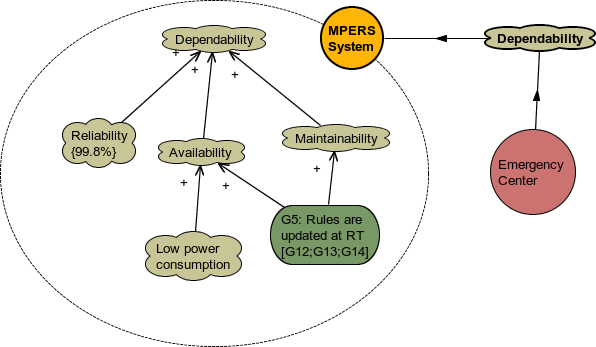
\includegraphics[width=0.6\textwidth]{imgs/MPERS_NFR.png}
\caption{MPERS non-functional requirements.}
\label{fig:MPERS_NFR}
\end{figure*}

%Intersting for motivation!
Some dependability attributes, similarly to the Awareness Requirements by Souza et al.~[AWREQ], define metrics over other requirements. These meta-requirements are not directly fulfilled by system functionalities like `emergency awareness' is fulfilled by `notify emergency' or `confidentiality' could be fulfilled by `user authentication', but by how these functionalities will perform. Reliability, for instance, is inversely proportional to the likelihood of failures. Thus, the reliability metric depends on the probability of system functionalities to fail. Conformity to these metrics is not implicit in the model, it requires some verification technique.

Each requirement in a goal model must come from another requirement through decomposition, means-end or contribution links, or it must be directly mapped to stakeholder needs through dependency links. Emergency center attended the patient's needs by providing and maintaining the MPERS system itself and by assuring other NFR for the system. Availability and reliability were selected as metrics over the system execution (meta-requirement), while maintainability is partially satisfied by the MPERS ability to update emergency rules at runtime and by other aspects that, for the sake of simplicity, we will omit in this evaluation.

It is not an easy task to define the exact constraint to these metrics. For instance, an analyst or a reliability engineer should be aware of what does it mean for a system to be 99.999\% reliable, as this level may not be achieved by any alternative solution and must be coherent to the system criticality - a catastrophic failure should be avoided by all means. In some cases, the system will have to comply to some industry standards or contract based constraints. Table~\ref{tab:MPERS_NFR} summarizes each quantitative NFR for MPERS.
\medskip

% Please add the following required packages to your document preamble:
% \usepackage{booktabs}
\begin{table}[h]\label{tab:MPERS_NFR}
{\renewcommand{\arraystretch}{1.5}
\begin{tabularx}{\textwidth}{@{}XXX@{}}
\toprule
\textbf{NFR}               & \textbf{Constraint} & \textbf{Target}        \\ \midrule
\textbf{Reliability}       & 99.8\%            & \textbf{G1} \\
\textbf{Power consumption} & 100 p.u.            & \textbf{G2}          \\ \bottomrule
\end{tabularx}
}
\caption{Non-functional metrics for the MPERS system.}
\end{table}

%softgoals of `continuous assistance' and `correct assistance'

As indicated by the \textit{Target} column, each NFR constraint may be associated to a root level goal or to any of its subgoals. The corresponding probabilistic verification based on the execution of a set of system tasks in the RGM is defined as:

\begin{itemize}

\item \textit{Global}, if the activities set is a minimum set composed of the tasks that satisfies the chain of subgoals up to the root goal Groot. For instance, in Table~\ref{tab:MPERS_NFR} reliability is (globally) required for the root goal G1.
\medskip

\item \textit{Local}, if the activities set is a minimum set composed of tasks that satisfies the chain of subgoals up to a goal Gx, where Gx != Groot. For instance, in Table~\ref{tab:MPERS_NFR} power consumption is (locally) required for the goal G2.
\medskip

\end{itemize}

%put here the formal definition of the root goal, subgoals, activity set, turple, etc

Other MPERS NFR are `emergency awareness' and `resources optimization'. These softgoals are addressed by system functionalities. The former receives a full contribution (double positive sign) from goal `emergency is notified', meaning it is fully satisfied by this goal. The later is just assumed to be partially satisfied by the `emergency is checked' functional goal.

\subsection{Non-functional requirements verification}


%NOT HERE!
%The probabilistic verification of systems with variability is not a novelty by itself. Many proposals have addressed this problem in the context of Dynamic Software Product Lines (DSPL), some of then using the PMC technique~[Vini, Paula, Who Else?]. In DSPL, optional and alternative features may be activated or deactivated at runtime. A family based verification of one or multiple NFRs, also called qualitative goals, indicates what combinations are valid or which combination is optimal.

This section describes the application of a PMC technique to verify the conformance of the RGM to defined non-functional constraints and also to solve the variability problem at design time considering both cases explained in Section~\ref{sec:variability}, i.e., for static context and dynamic contexts.

\subsubsection{The DTMC model}

%It is not always the case that multiple alternatives must be evaluated and compared. A goal model may be built with only mandatory goals, dependencies and tasks. Nonetheless, non-functional constraints may still have to be checked, i.e., a single alternative verification may have to be performed. 

The state-based verification of meta-requirements or non-functional constraints that specifies how different functionalities should perform is a complex task that involves a representation of system states and their transitions. A goal model may define system requirements with variable abstraction levels. As such, the feasibility of the verification of a given metric depends on the information provided by the model.

The MPERS RGM in Figure~\ref{fig:MPERS_LR} expands its main goals in further subgoals that are ultimately satisfied by means-end tasks. Some tasks are themselves decomposed into more granular subtasks. In our proposal, leaf-tasks are mapped to modules in the DTMC model. In PRISM, modules are containers for variables and commands, i.e., for states and behaviour. Figure~\ref{fig:PRISM_TASK_MODULE} presents a high-level representation of a system task as a PRISM module.

\begin{figure*}[ht]
\centering
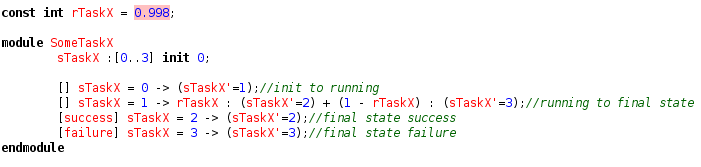
\includegraphics[width=1\textwidth]{imgs/PRISM_TASK_MODULE.png}
\caption{A PRISM DTMC module representing a system task.}
\label{fig:PRISM_TASK_MODULE}
\end{figure*}

In Figure~\ref{fig:PRISM_TASK_MODULE}, variable sTask indicates the state of some task. Different states of a task's life cycle are mapped to the value of this variable, namely: init (0), running (1), success (2) and failure (3). Success and failure are the final absorbing states for a task instance. Transition to these states is conditioned to the rTask probability: the closer this variable is to 1, the higher the probability of reaching the success state. 

Given a set of leaf-tasks that fulfils a chain of subgoals until a certain goal G and a reliability constraint defined as the probability of successfully achieving this goal, a DTMC model composed of modules for each leaf-task states and transitions is build. This model must represent the same workflow defined by the corresponding runtime goal model. Figure~\ref{fig:CRGM_TO_DTMC} illustrates this process.

\begin{figure*}[ht]
\centering
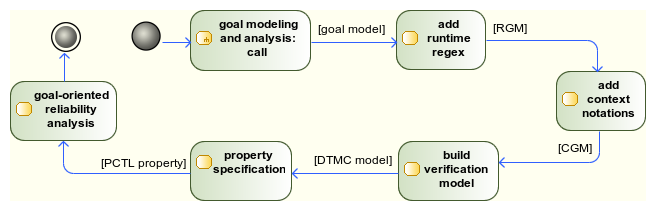
\includegraphics[width=0.75\textwidth]{imgs/CRGM_TO_DTMC.png}
\caption{Building a DTMC model from a contextual/runtime goal model.}
\label{fig:CRGM_TO_DTMC}
\end{figure*}

\subsubsection{RGM to DTMC}

Each task starts at a discrete time slot. Time slots defines the sequence order of tasks executions. Interleaved tasks (T1\#T2) have their initial state transition synchronized at the same time slot through labels, but occupy different time paths, i.e., following transitions are interleaved. Sequential tasks (T1;T2) have subsequent time slots, meaning that T2's initial transition is synchronized to T1's success transition. Table~\ref{tab:MPERS_DTMC_SLOTS} presents the time slots, paths and other dynamic aspects of MPERS leaf-tasks.

% Please add the following required packages to your document preamble:
% \usepackage{booktabs}
\begin{table}[h]\label{tab:MPERS_DTMC_SLOTS}
{\renewcommand{\arraystretch}{1.5}
\begin{tabularx}{\textwidth}{@{}lllllll@{}}
\toprule
\textbf{Task}  & \textbf{Time path} & \textbf{Time slot} & \textbf{Optional} & \textbf{Conditional} & \textbf{Alternative} & Cardinality \\ \midrule
\textbf{T15}   & 0                  & 0                  & false             & false                & false                & 1           \\
\textbf{T16}   & 0                  & 1                  & false             & false                & false                & 1           \\
\textbf{T17.1} & 0                  & 2                  & false             & false                & false                & 1           \\
\textbf{T17.2} & 0                  & 3                  & true              & false                & false                & 1           \\
\textbf{T18}   & 0                  & 4                  & false             & false                & false                & 1           \\
\textbf{T19.1} & 0                  & 5                  & false             & false                & false                & 1           \\
\textbf{T19.2} & 0                  & 6                  & false             & false                & false                & 1           \\
\textbf{T20}   & 0                  & 7                  & false             & false                & false                & 1           \\
\textbf{T21}   & 1                  & 7                  & false             & false                & false                & 1           \\
\textbf{T9.1}  & 2                  & 7                  & false             & false                & T9.2                 & 1           \\
\textbf{T9.2}  & 2                  & 7                  & false             & false                & T9.1                 & 1           \\
\textbf{T22}   & 0                  & 8                  & false             & false                & T24                  & 2           \\
\textbf{T23}   & 0                  & 9                  & false             & false                & T24                  & 1           \\
\textbf{T24}   & 3                  & 8                  & false             & false                & T22                  & 1           \\
\textbf{T25}   & 3                  & 9                  & false             & false                & T22                  & 1           \\
\textbf{T13.1} & 4                  & 0                  & false             & false                & false                & 1           \\
\textbf{T13.2} & 4                  & 0                  & false             & false                & false                & 1           \\
\textbf{T13.3} & 4                  & 0                  & false             & false                & false                & 1           \\ \bottomrule
\end{tabularx}
\caption{Dynamic aspects of the MPERS leaf-tasks in the DTMC model.}
}
\end{table}

Other possible behaviours are: alternative execution (E1|E2), optional execution (opt(E1)) and conditional execution (try(E)?E1:E2). For alternative OR decomposition, or XOR, a parameter in the model should decide which alternative from a set of two or more is selected for analysis. Only one alternative should be enabled at a time. Similarly, optional tasks are enabled by a boolean variable. Finally, labels are used to condition the execution of tasks to the success and failure of a third task. 

Cardinality is also supported by the runtime regex specification. In our proposal, execution cardinality is simply represented by n modules with subsequent time slots (E+n) or by modules whose initial transition are synchronized and following transitions are interleaved (E\#n). Figures~\ref{fig:PRISM_ALT_TSKS, fig:PRISM_OPT_TSK, fig:PRISM_COND_TSK} illustrate different tasks behaviours.

\begin{figure*}[ht]
\centering
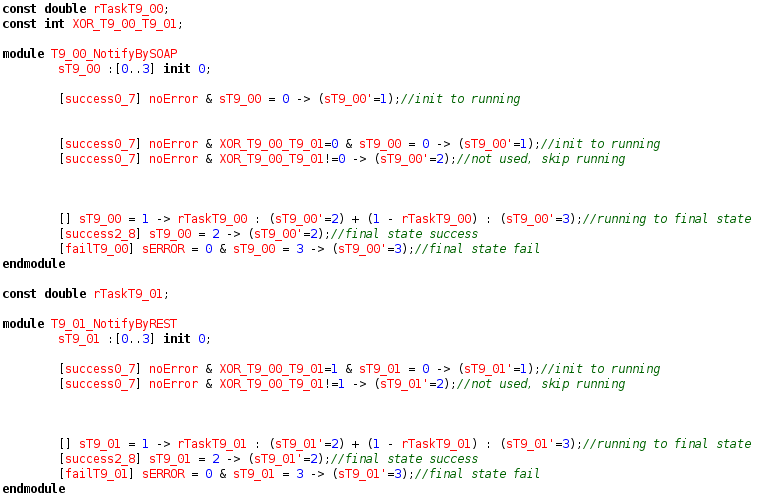
\includegraphics[width=1\textwidth]{imgs/PRISM_ALT_TSKS.png}
\caption{Alternative tasks T9.1 and T9.2 as DTMC modules.}
\label{fig:PRISM_ALT_TSKS}
\end{figure*}

\begin{figure*}[ht]
\centering
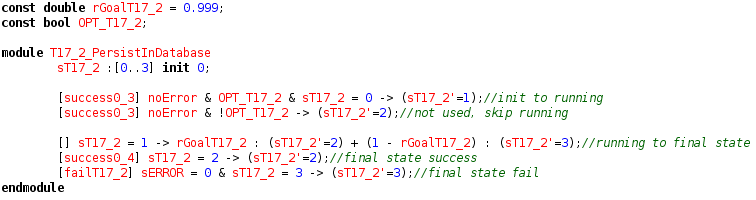
\includegraphics[width=1\textwidth]{imgs/PRISM_OPT_TSK.png}
\caption{An optional task T17.2 as a DTMC module.}
\label{fig:PRISM_OPT_TSK}
\end{figure*}

%Listing~\ref{ls:MPERS_DTMC} presents the DTMC model for the MPERS.

%To illustrate our proposal for NFR verification of a single alternative, we selected the local goal G5 that defines the state where emergency rules are updated without major system interruption. Table~\ref{tab:MPERS_NFR} has a non-functional constraint for this goal that specifies the minimum 

\subsubsection{Variability in GORE}

The variability in goal models leads to more than one minimum set of tasks capable of fulfilling local or root goals. In OR-decomposition, at least one alternative is required and the maximum number of combinations is defined by $1 + 2^{(n-1)}$, with n the number of OR-decomposed goals/tasks. Therefore, the individual verification of all alternatives in a goal model may prove to be inefficient if too many variation points exist in the model.

The PMC approach has already been explored for the verification of models with variability. Rodrigues et al. proposed a family-based verification of software product lines (SPL)~[RODRIGUES]. The main idea is to reduce the analysis effort and boost the feasibility of the SPL verification. Parameters in a PRISM probabilistic model generates a parametric formula for all products in the SPL for a given PCTL property. 

In our proposal, PCM verification follows the same principle of the SPL family-based verification. A parametric formula should be generated from the RGM. Alternatives are selected by passing values to parameters. For instance, if both SOAP and REST are available means for remote emergency notification, a parameter with values 0 or 1 will indicate which alternative is enabled for verification. Eq.~\ref{eq:MPERS_RELIABILITY_FORM} defines the reliability formula for the root goal G1.

\begin{equation}
G1r=c^2\label{eq:MPERS_RELIABILITY_FORM}
\end{equation}

A family-based PMC is useful for comparing each alternative with non-functional metrics as criteria to decide which one should be used by the system-to-be at design time or by the real system at runtime. At design time, this approach is analogue to the TROPOS contribution analysis. In both cases, a unique parametric formula evaluates a PCTL property corresponding to a non-functional metric.  %improve the example!


% or the verification tool should decide based on some probabilistic distribution setted by the analysts (probabilistic alternative selection, or PAS).

%In contrast, PAS provides verification for systems that include variability in its design. The verification of NFR metrics for these systems depend on how each alternative is selected during system operation.

\subsubsection{Context selection}

As in the contextual goal model, contexts may limit which alternatives are adoptable. This effect must be considered in a realistic verification. As a novelty, our approach for the verification of non-functional metrics through PMC will also include variable contexts of operation and their effects in the verification model. Two different approaches for context selection may be employed: 

\begin{itemize}

\item \textit{Deterministic context selection, or DCS}: one context is selected by the analyst before the verification. Context effects in the verification model should be activated and cause the evaluation result to correspond to the selected context.
\medskip

\item \textit{Probabilistic context selection, or PCS}: a probability distribution will define the likelihood of a context to be selected and the corresponding context implications in the verification model to be activated.  

\end{itemize}

Both approaches are complementary as the first verifies the selected alternative for one context at a time and the last verifies a realistic scenario with multiple possible contexts. 

\subsubsection{Context-alternative selection}

Table~\ref{tab:DAS_PAS_DCS_PCS} summarizes each verification approach and possible combinations.

% Please add the following required packages to your document preamble:
% \usepackage{booktabs}
\begin{table}[h]\label{tab:DAS_PAS_DCS_PCS}
{\renewcommand{\arraystretch}{1.5}
\begin{tabularx}{\textwidth}{@{}l|XXX@{}}
\toprule
             &                                                         & \textbf{DAS}                                                                                                      & \textbf{PAS}                                                                                                     \\ \midrule
             &                                                         & A single alternative is selected by the analyst.                                                                  & Alternative selection follows a probabilistic distribution.                                                      \\
\textbf{DCS} & An unique context is selected by the analyst.           & Alternative selection by the analyst is limited by the selected context.                                          & Probabilistic alternative selection is limited by the selected context.                                          \\
\textbf{PCS} & Context selection follows a probabilistic distribution. & Alternative selection by the analyst may fail according to the probability of selecting an incomplatible context. & Probabilistic alternative selection may fail according to the probability of selecting an incomplatible context. \\ \bottomrule
\end{tabularx}
}
\caption{Description of the different approaches for verifying a system with variable alternatives and variable contexts.}
\end{table}

If the context selection is deterministic (DCS), there is no reason for verifying an alternative that is known to be incompatible with the selected context. Therefore, only adoptable alternatives must be verified. In opposition, if context selection is probabilistic, that alternative may still be valid in other contexts, hence it must be included in the multi-context evaluation. For instance, the patient location identification through GPS (alternative) will certainly fail if the GPS signal is not available (context). Thus, the DAS-DCS combination checks one compatible context-alternative pair at a time, while DAS-PCS combination leads to the verification of multiple context-alternative pairs at the same time.

The idea behind a probabilistic context selection is to emulate a realistic scenario in which the context of operation varies and the system must avoid requirements violations by  having an adoptable alternative for each context. This holistic evaluation provides measures weighted by the probabilistic context distribution. For instance, if GPS signal is available 70\% of the time and triangulation is available 90\% of the time and if each method has its own reliability, namely rGPS and rTRI, the reliability of high-level task `identify patient location' is defined by the expression 0.9*rGPS + 0.1*0.7*rTRI, considering that GPS has priority over triangulation. 


\subsubsection{Discrete-time Markov chain model}



\subsubsection{Reliability verification}

Transition probability between running to final success state is described by the individual reliability of the corresponding task, namely rTask. 

\subsubsection{Power consumption verification}

%The same principle is applied to the PAS combinations. Incompatible alternatives are removed from the selection list if the context for which they are incompatible is fixed. Or, if context selection is probabilistic, for each context the verification model should be able to avoid the probabilistic selection of incompatible alternatives. This simulates the self-adaptive capability of systems that are designed to tolerate context changes.

%This section is divided in preliminary conceptual explanation about the

\subsection{Probabilistic model generation}

In the PMC technique that has been adapted by this proposal, a behavioural specification, usually provided by UML activity and sequence diagrams, are manually converted to a probabilistic model in PRISM language. This tends to be a costly and error-prone process with a complexity proportional to the number of components, actions and interactions causing state transitions.  

As a goal model is traversed from strategical root goal to operational leaf-goals, and each leaf-goal is reachable by a delegation to other actor or by a operational task, then a behaviour specification as proposed by the RGM may have enough information to be consumed as input for the generation of probabilistic models in PRISM language and for the verification of some important NFRs. However, the manual generation from RGM is still a costly task.

Depending on the abstraction level and the nature of the verification, PRISM models may either very complex or may follow a clear pattern. For instance, PRISM modules can be used to represent leaf-tasks of a runtime goal model. Considering a DTMC model, a task workflow can be modelled as a sequence of probabilistic state transitions according to the behavioural specification parsed from the RGM. This probabilistic model follows a pattern that motivated the implementation of an automatic generation of DTMC models representing leaf-tasks execution directly from a runtime goal model.

Leaf-tasks are not necessarily atomic system tasks. The idea is to leave to analysts the decision concerning the abstraction level represented by the tasks that will be verified. For instance, the abstract task `find active sensors' could be decomposed in more granular and concrete tasks related to the platform, architecture and language used for implementation. 

The more abstract a task is, the more difficult is to obtain their individual metrics, as the trace between an abstract and the concrete system operation becomes less evident. Any NFR verification by the PMC technique requires further qualitative information about individual parts involved in an activity, e.g., the reliability, performance, power consumption, cost and other attributes for tasks in a workflow or for components involved in a task.

This is a key point in this approach, as it may seen too loose to couple a probabilistic verification to a goal model with a high-level operational representation of a system. But its feasibility becomes clear when the metrics being verified are compatible with the abstraction level of the tasks and information regarding how each task individually performs is available or can be collected.


\subsection{From NFR to PCTL properties}

The estimation of attributes through PMC technique is limited to those that a probabilistic model may evaluate. Dependability attributes have an abstract definition that must be associated to a concrete and verifiable PCTL property. To demonstrate our approach, we verify the MPERS model for the following attributes:

\begin{itemize}

\item \textbf{Reliability}, represented by the probability of a successful execution of all the activities involved in fulfilling leaf-goals of a certain system alternative. It is also know as the \textit{reachability} as the describes the probability of reaching a final and successful system state. 
\bigskip

\item \textbf{Availability}, represented by the power consumption estimation to maximize the time that the system will remain operational depending only on its battery. This attribute is well related to mobile computing. 
\medskip

\end{itemize}


each task has its own states, including the failure and the success states. Many factors may contribute to the correctness or the failure of system tasks, including internal and external events. The probability of a successful task execution defines its reliability. 

In a complex workflow of tasks with different rel 

In order to be successful, tasks depend on the proper interaction among the components 

seen as an activity diagram and be used to generate a probabilistic model in PRISM language. This allows the model checking of the corresponding goal model as a set of activities for which temporal and other behaviour aspects are specified by the runtime regex of the RGM.

\section{Treating NFR Violations}

\begin{itemize}

\item Making a different choice for underlying components: In some cases the replacement of a technical component for another of the same class can improve the quality of how they achieve their goal. For instance,
\medskip

\item Behaviour optimization: The quality may also depend on the pattern used for the activities execution. The specification of a different pattern may eliminate the non-functional violation. 
\medskip

\item Contextualizing the alternative: An alternative may only violate a NFR in specific contexts. In this case, different valid alternatives may be used according to the context of operation.
\medskip

\item Alternative disposal: If the alternative is in absolute violation or if its validity is restricted to contexts that have at least one other valid alternative, this branch can be eliminated from the model.

\end{itemize}

Dependability analysis is used to provide information about different dependability attributes related to system failures. These metrics may be specified as non-functional requirements for isolated system functionalities or for the whole system. Instead of softgoals, we use meta-requirements over functional goals with clear-cut quantitative criteria such as `99.999\%' reliable - a probabilistic value to make it compatible with the PMC estimation results.

To perform the , we focus on dependability related metrics that should be estimated and compared to their required constraint values through quantitative analysis. Sensitive analysis to reveal how different system parts contribute to the overall value of those attributes. Sensitive analysis may be considered analogous to the original GORE contribution analysis.



\section{TROPOS to PMC Code Generation}

As we wanted to automate the code generating process for the verification model, the graphical modelling environment that supports TROPOS methodology and the code generation for multi-agents was extended to also generate probabilistic models for the PMC technique.

To reduce the effort of codifying the verification model, an automated generation of the PRISM probabilistic model was implemented based on an existing open source tool for TROPOS development support named TAOM4E[citation]. TAOM4E provides a graphical environment for goal modelling with TROPOS methodology based on the well known Eclipse Modelling Framework (EMF) and Graphical Editing Framework (GEF). The GORE to PRISM generator was implemented as a Eclipse plugin and integrated to the TAOM4E environment. 

The purpose  of the automated code generation for the probabilistic PRISM model is to optimize the formal verification step by abstracting the PRISM language from the analysts and reduce the overhead and time of the model verification. This should increase the feasibility of adopting the extended TROPOS methodology by keeping analysts with their original responsibility of modelling and analysing the system, its social environment and its different contexts of operation.





In terms of a high level system behaviour, each activity has its own states space including success and failure. Our probabilistic verification approach requires not only a formal specification of the system behaviour, but also metrics related to how individual components involved in system activities will perform in respect to the analysed metric. In reliability verification, each component has an individual probability of successfully performing its functional task. Analysts must obtain these values by consulting their manufacturer, by individually analysing each component reliability based on their behaviour specification until the atomic level or by monitoring these components in a testing or production environment. Further details of how individual metrics may be obtained for the PCM may be found at the literature and are out of the scope of this work.
